% !TeX program = xelatex
% !TeX encoding = utf8
% !TeX root = Elo1_HS22.tex

%% TODO: publish to CTAN
\documentclass[margin=normal]{tex/hsrzf}

%%%%%%%%%%%%%%%%%%%%%%%%%%%%%%%%%%%%%%%%%%%%%%%%%%%
% Packages

%% TODO: publish to CTAN
\usepackage{tex/hsrstud}

%% Language configuration
\usepackage{polyglossia}
\usepackage{multicol}
\usepackage{tikz}
\usepackage[european]{circuitikz}
\usepackage{tabularx}
\setdefaultlanguage[variant=swiss]{german}

%% License configuration
\usepackage[
    type={CC},
    modifier={by-nc-sa},
    version={4.0},
    lang={german},
]{doclicense}

%%%%%%%%%%%%%%%%%%%%%%%%%%%%%%%%%%%%%%%%%%%%%%%%%%%
% Metadata

\course{Elektrotechnik}
\module{Elo1}
\semester{Herbstsemester 2022}

\authoremail{joel.leirer@ost.ch}
\author{\textsl{Joël Leirer} -- \texttt{\theauthoremail}}

% did someone help you with this work?
\contributors{

  % do not forget to add yourself!
}

\title{\texttt{\themodule} Zusammenfassung}
\date{\thesemester}

%%%%%%%%%%%%%%%%%%%%%%%%%%%%%%%%%%%%%%%%%%%%%%%%%%%
% Document

\begin{document}

% use roman numberals for introductiory pages
\pagenumbering{roman}

\maketitle

% \begin{abstract}
% \end{abstract}

% show the names of the people who contributed to this document.
% \section*{Contributors}
% \thecontributors

\section*{Lizenz}
\doclicenseThis

\clearpage
\tableofcontents

% actual content
\clearpage
\setcounter{page}{1}
\pagenumbering{arabic}

\section*{NOTE}
Erlaubte Unterlagen an Prüfung: 5x A4-Seiten Zusammenfassung, Taschenrechner
\section{Arbeitspunktbestimmung}
AC und DC Teile der Schaltung separat anschauen.
\begin{multicols}{2}

  \subsection{DC}
  \begin{itemize}
    \item Grosssignalwiderstung ($\frac{U}{I}$)
    \item AC-Quellen "Abschalten", AC-Quellen mit DC Anteil durch DC-Quellen ersetzen
    \item Kondensatoren entfernen (Unterbruch)
    \item Spule Kurschliessen
  \end{itemize}
  \subsection{AC}
  \begin{itemize}
    \item Kleinsignalwiderstand (Impedanz,$\frac{dU}{dI}$ )
    \item DC-Quellen "Abschalten"
    \item Nichtlineare Bauteile durch ihre Kleinsignal Ersatzschaltung ersetzen
    \item Kondensatoren kurzschliessen
    \item Sperrdrosseln ("grossse" Induktivitäten) entfernen (Unterbruch)
  \end{itemize}
\end{multicols}

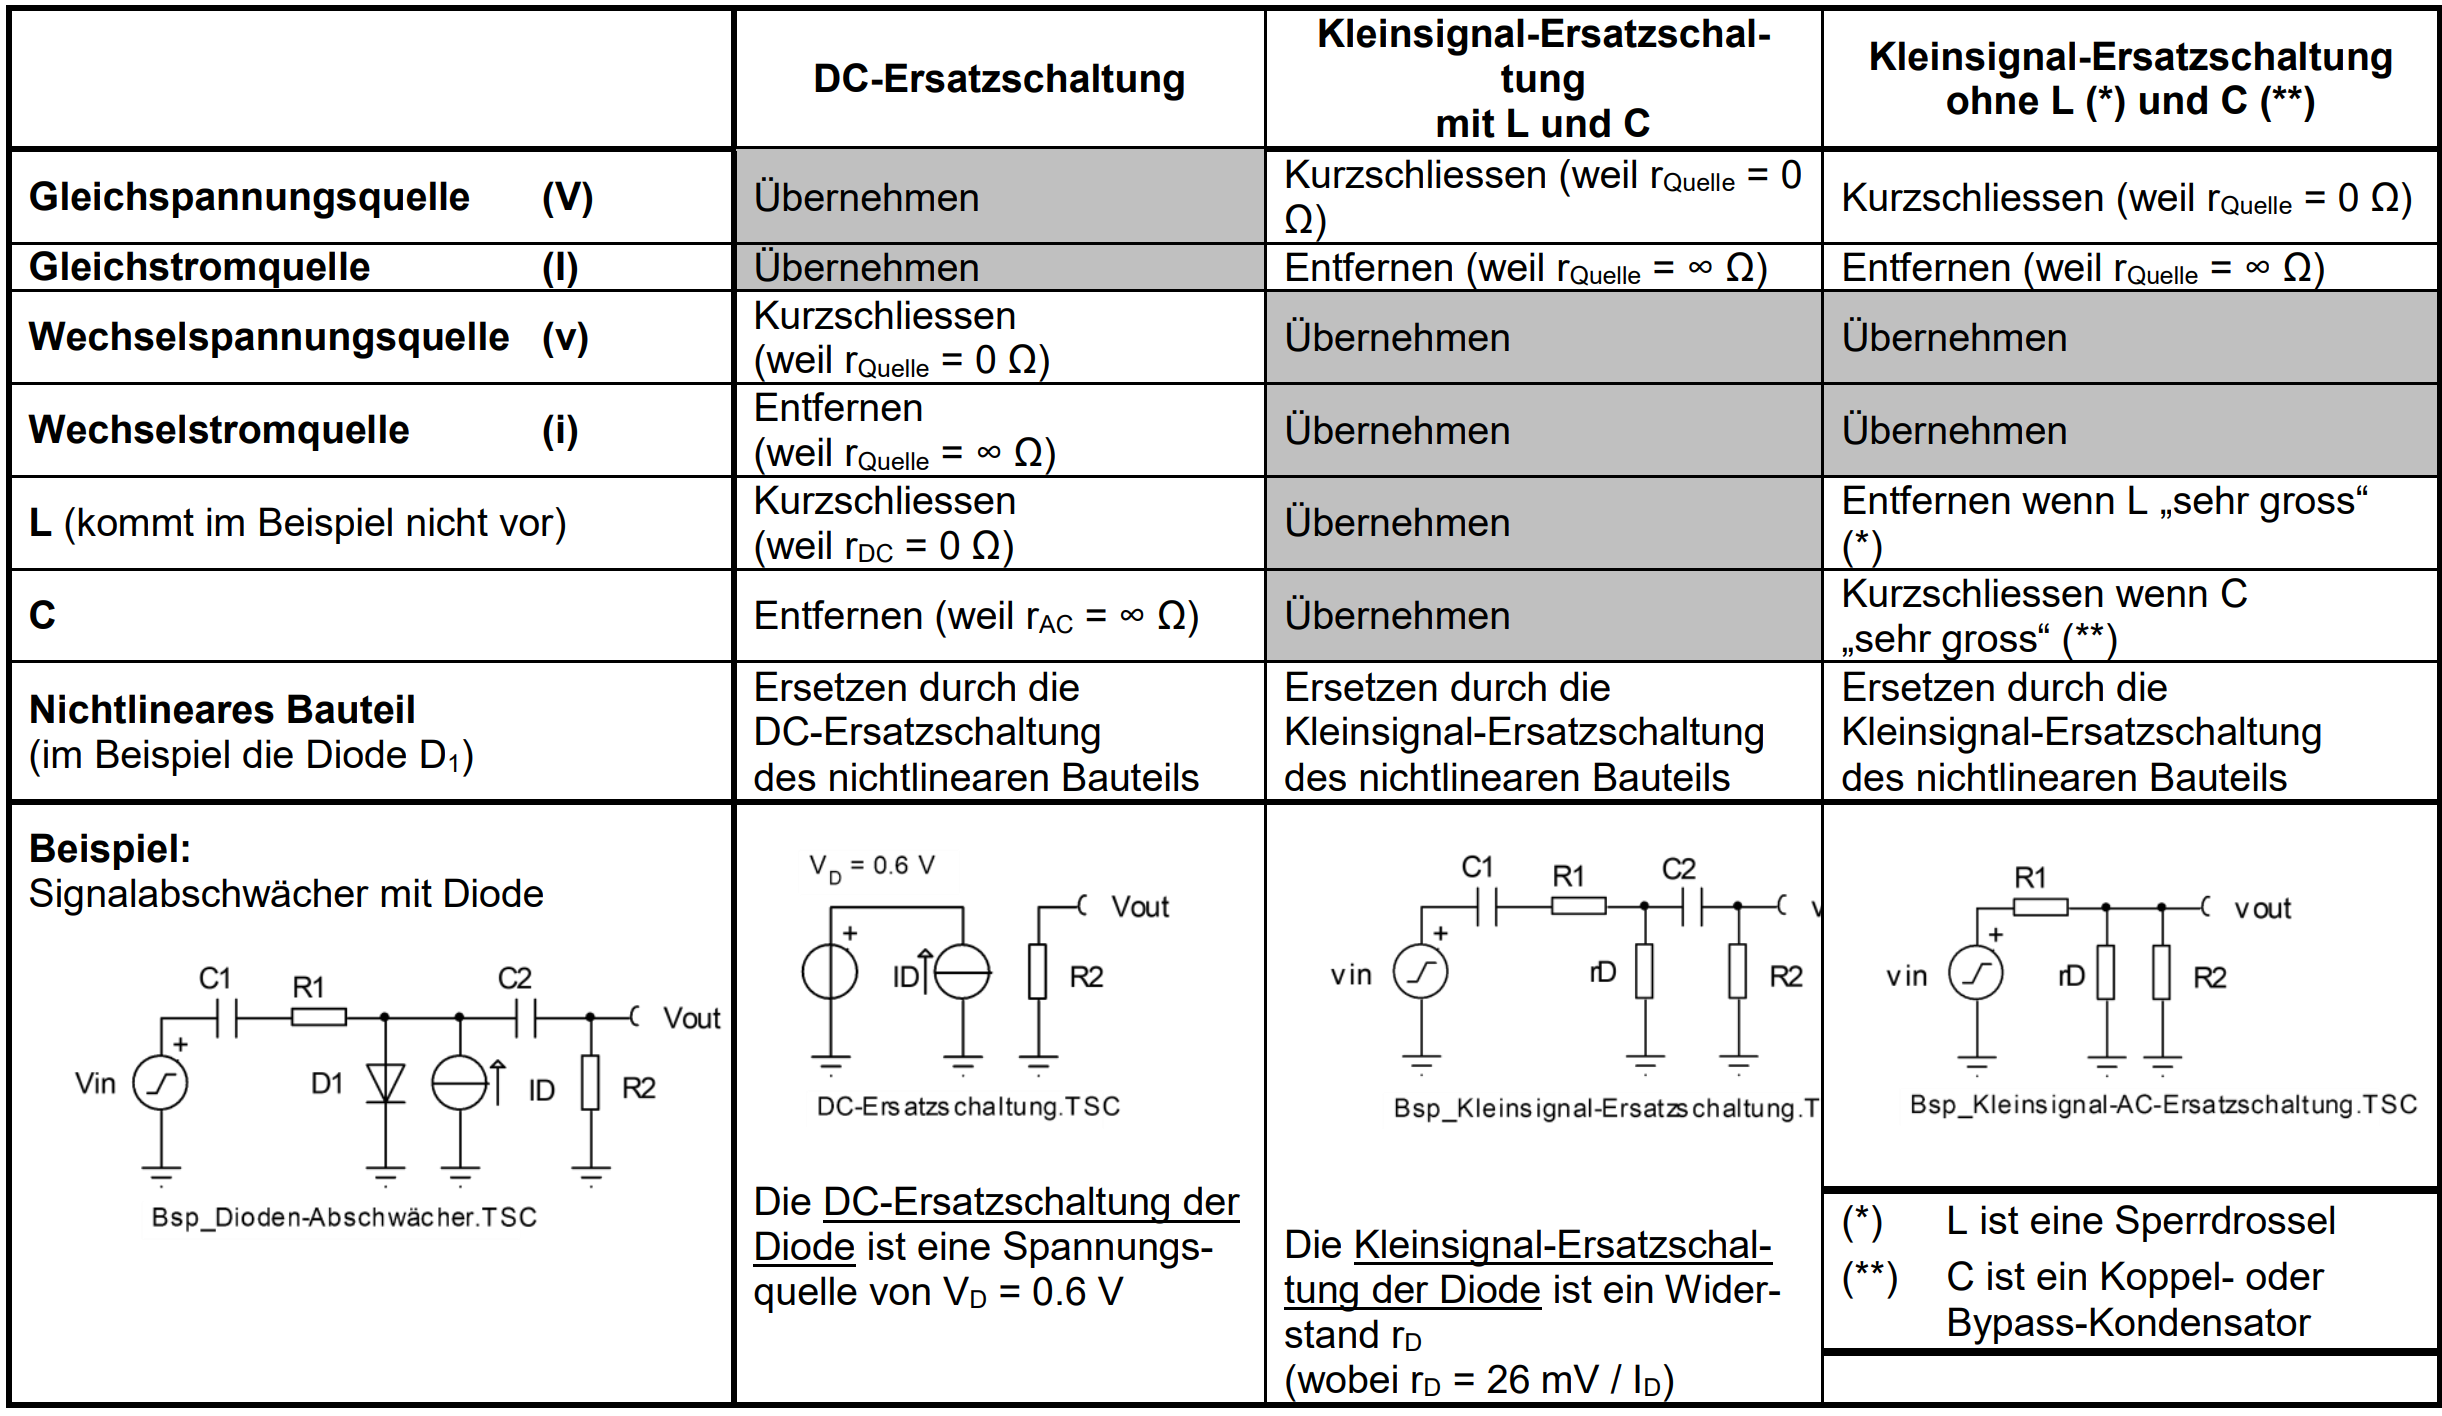
\includegraphics[width = 15cm]{img/Tabelle Kleinsignal Ersatzschaltung.png}

\section{OpAmp}
\subsection{Schaltungen mit negativer Rückkopplung}
\begingroup
  \small
  \begin{tabularx}{0.8\textwidth}{p{155pt}p{155pt}p{155pt}}
    \textbf{Nicht Invertierender Verstärker}                                                          &
    \textbf{Invertierender Verstärker}                                                                &
    \textbf{Summierender Verstärker}                                                                    \\
    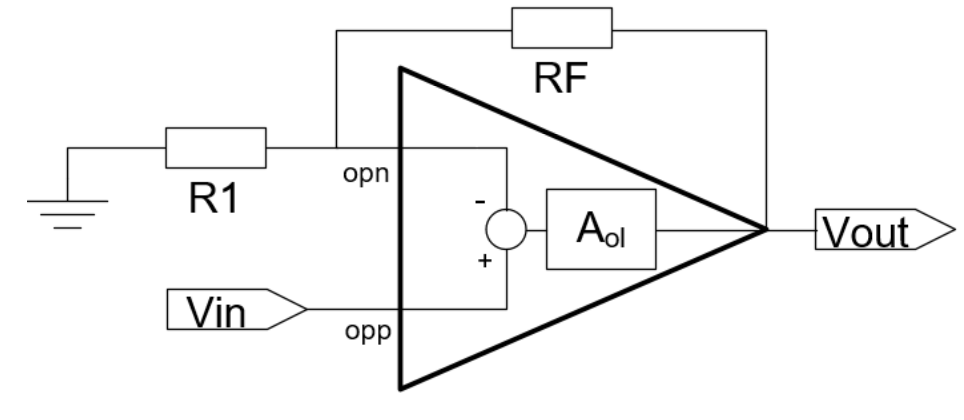
\includegraphics[width = 3.5cm]{img/OpAmp/Verstaerker_nicht_invertierend.png}                     &
    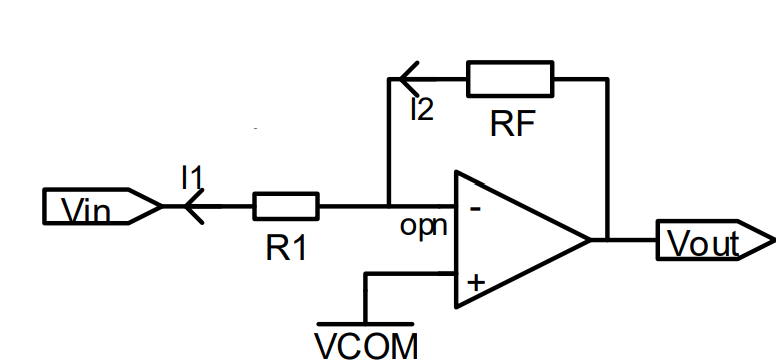
\includegraphics[width = 3.5cm]{img/OpAmp/Verstaerker_invertierend.png}                           &
    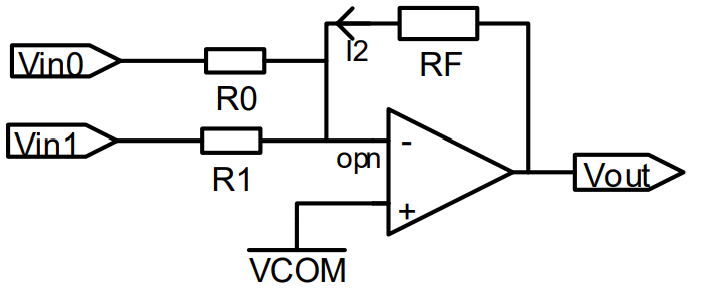
\includegraphics[width = 3.5cm]{img/OpAmp/Verstaerker_summierend.png}                               \\
    $ V_{out} = \frac{1}{\frac{R_1}{R_1 + RF} (+ \frac{1}{A_{ol}})} \cdot V_{in} $                    &
    $ V_{out} = V_{RF} = -\frac{RF}{R_1}\cdot V_{in}$                                                 &
    $ V_{out} = RF \cdot I_2 = -RF \cdot (\frac{V_{in1}}{R_1} + \frac{V_{in0}}{R_0}) $                  \\
    \textbf{Buffer}                                                                                   &
    \textbf{Invertierender Addierer}                                                                  &
    \textbf{Gewichteter Subtrahierer}                                                                   \\
    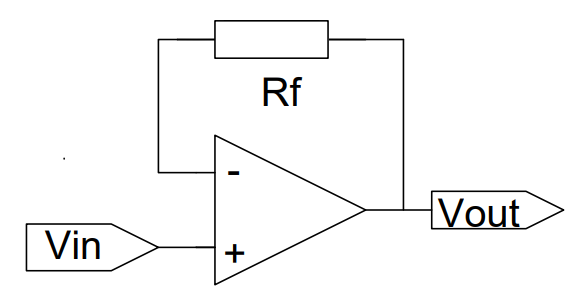
\includegraphics[width = 3.5cm]{img/OpAmp/Buffer.png}                                             &
    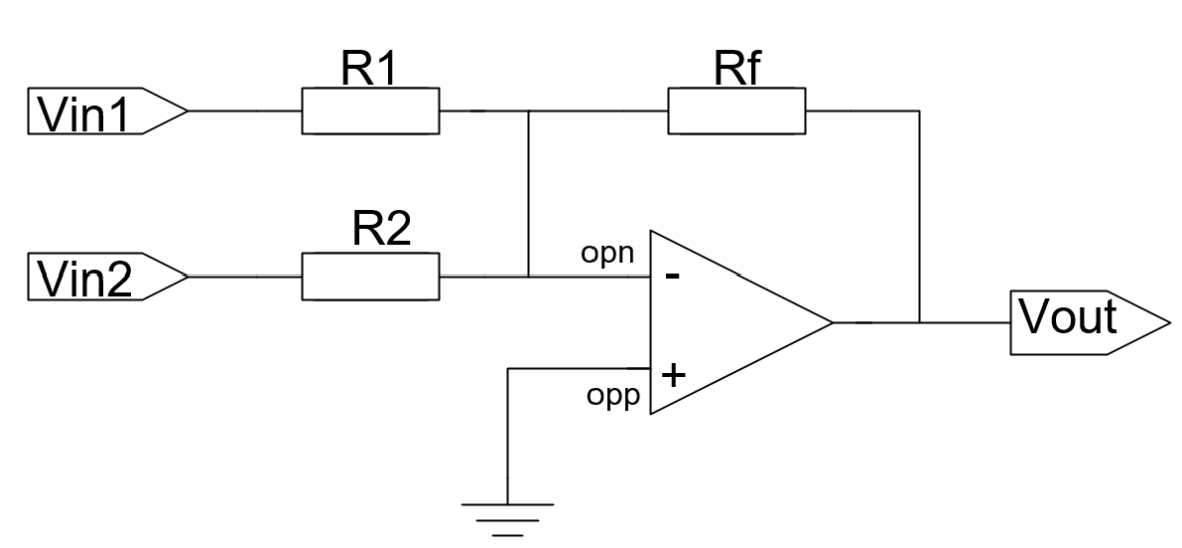
\includegraphics[width = 3.5cm]{img/OpAmp/Invertierender_Addierer.png}                            &
    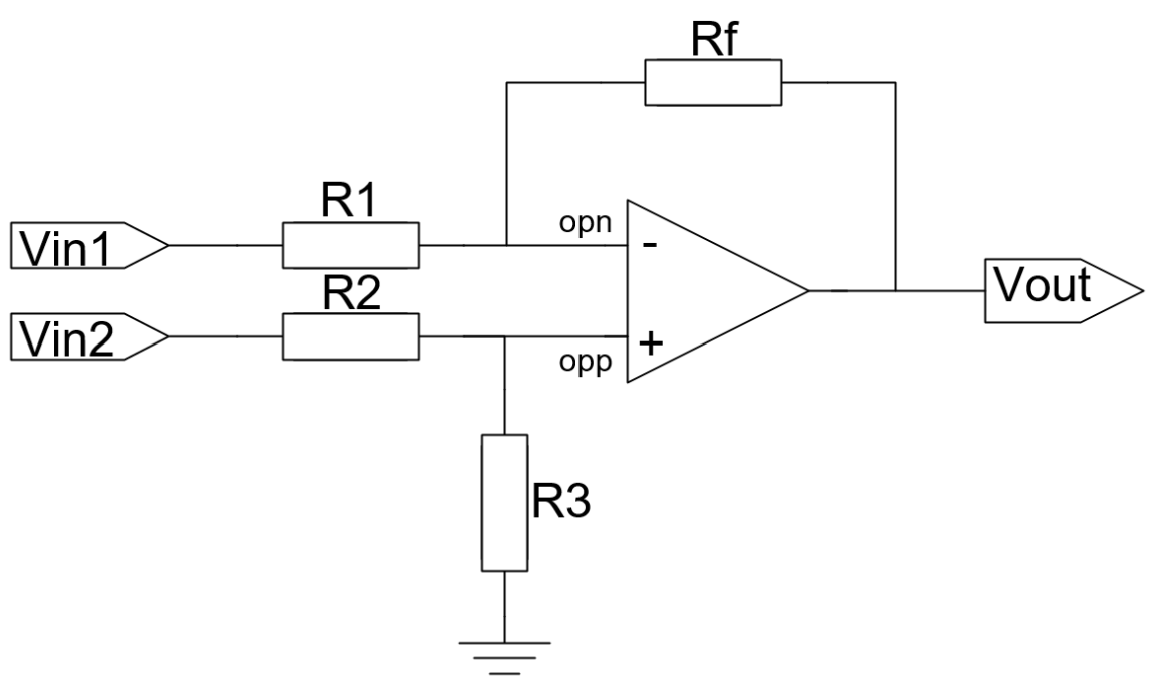
\includegraphics[width = 3.5cm]{img/OpAmp/Gewichteter_Subtrahierer.png}                             \\
    $ V_{out} = V_{in}$                                                                               &
    $ V_{out} = - RF \cdot (\frac{V_{in1}}{R_1} + \frac{V_{in2}}{R_2}) $                              &
    $ V_{out} =-\frac{RF}{R_1} \cdot V_{in1} $                                                          \\
    \textbf{Differenzverstärker}                                                                      &
    \textbf{Instrumentenverstärker}                                                                   &
    \textbf{Mehrstufige Verstärker}                                                                     \\
    \\
    \includegraphics[width = 3.5cm]{img/OpAmp/Differenzverstärker.png}                                &
    \includegraphics[width = 3.5cm]{img/OpAmp/Instrumentenverstärker.png}                             &
    \includegraphics[width = 3.5cm]{img/OpAmp/Mehrstufige_Verstärker.png}                               \\
    \\
    $ V_{out} = V_{AGND} + \frac{R_4}{R_3} \cdot(V_{in1} - V_{in2}) $                                 &
    $ V_{out} = V_{ref} + \frac{R_4}{R_3} \cdot (1 + \frac{Rf1 + Rf2}{RG}) \cdot (V_{in1} - V_{in2})$ &
    Verstärkung total $ A_{tot} = A_1 \cdot A_2 \cdot A_3\cdot\dots$                                    \\
    \textbf{Invertierender Verstärker \newline
    mit T-Glied in Rückkopplung}                                                                      &
    \textbf{Negativer Impedanz Konverter NIC}                                                         &
    \\
    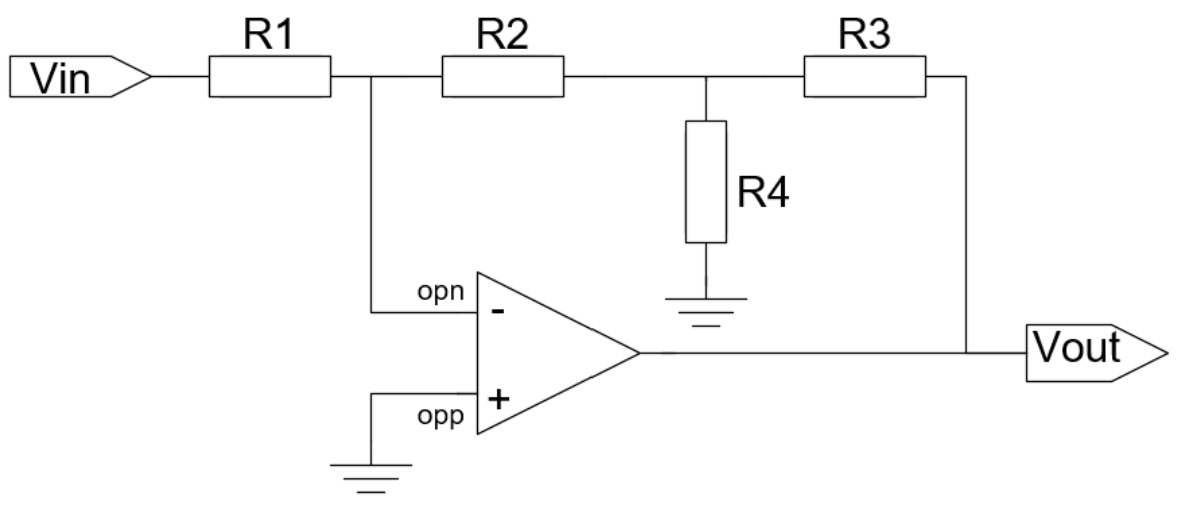
\includegraphics[width = 3.5cm]{img/OpAmp/Invertierender_Verstärker_mit_T-Glied_Rückkopplung.png} &
    \includegraphics[width = 3.5cm]{img/OpAmp/Negativer_Impedanz_Verstärker.png}                      &
    \\
    $ V_{out} = - V_{in} \cdot \frac{R_2 + R_3 + \frac{R_2R_3}{R4}}{R_1} $                            &
    $ V_{out} = V_{in} \cdot (1+ \frac{R_2}{R_1})$                                                    &
    \\
  \end{tabularx}
\endgroup

\subsubsection{Gesteuerte Quellen}
\begingroup
  \small
  \begin{tabularx}{0.8\textwidth}{p{100pt}p{100pt}p{100pt}p{120pt}}
    \textbf{Spannungsgesteuerte \newline Stromquelle V1}                                         &
    \textbf{Spannungsgesteuerte \newline  Stromquelle V2}                                        &
    \textbf{Spannungsgesteuerte \newline Stromquelle \newline
    für geerdete Last RL}                                                                        &
    \textbf{Stromgesteuerte \newline Stromquelle}                                                           \\
    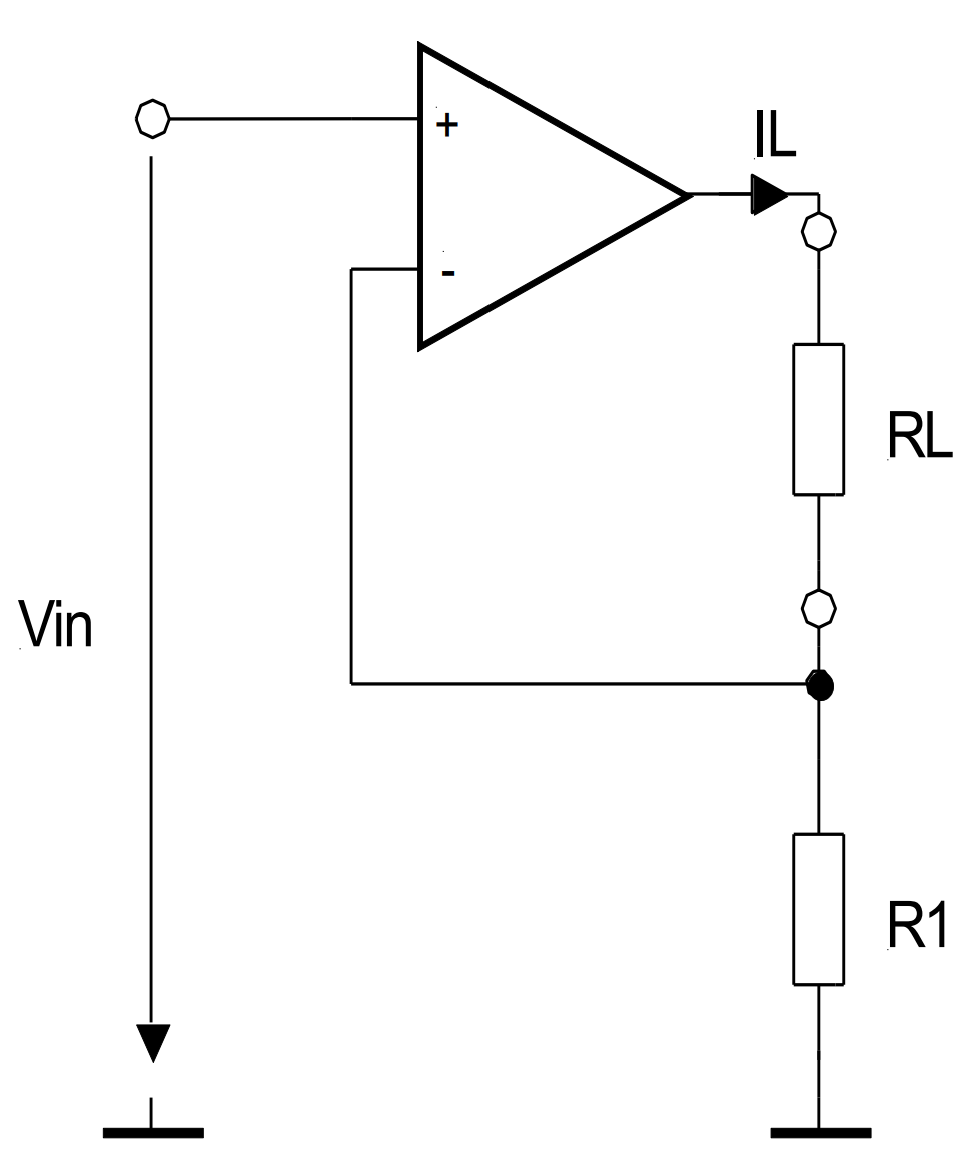
\includegraphics[width = 3.5cm]{img/OpAmp/Spannungsgesteuerte_Stromquelle_V1.png}            &
    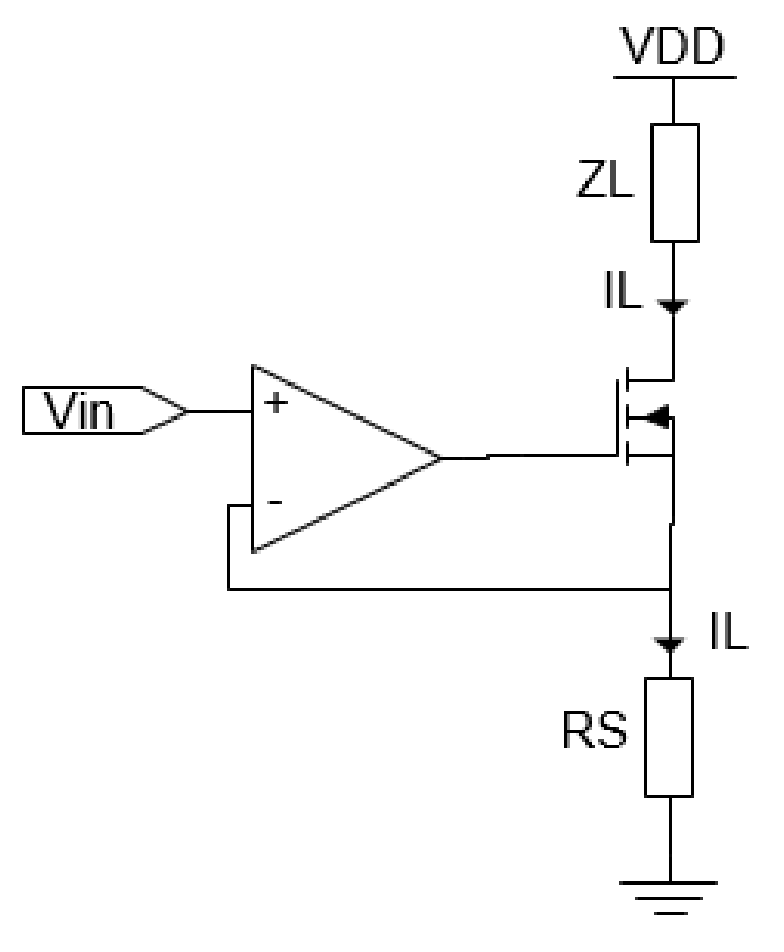
\includegraphics[width = 3.5cm]{img/OpAmp/Spannungsgesteuerte_Stromquelle_V2.png}            &
    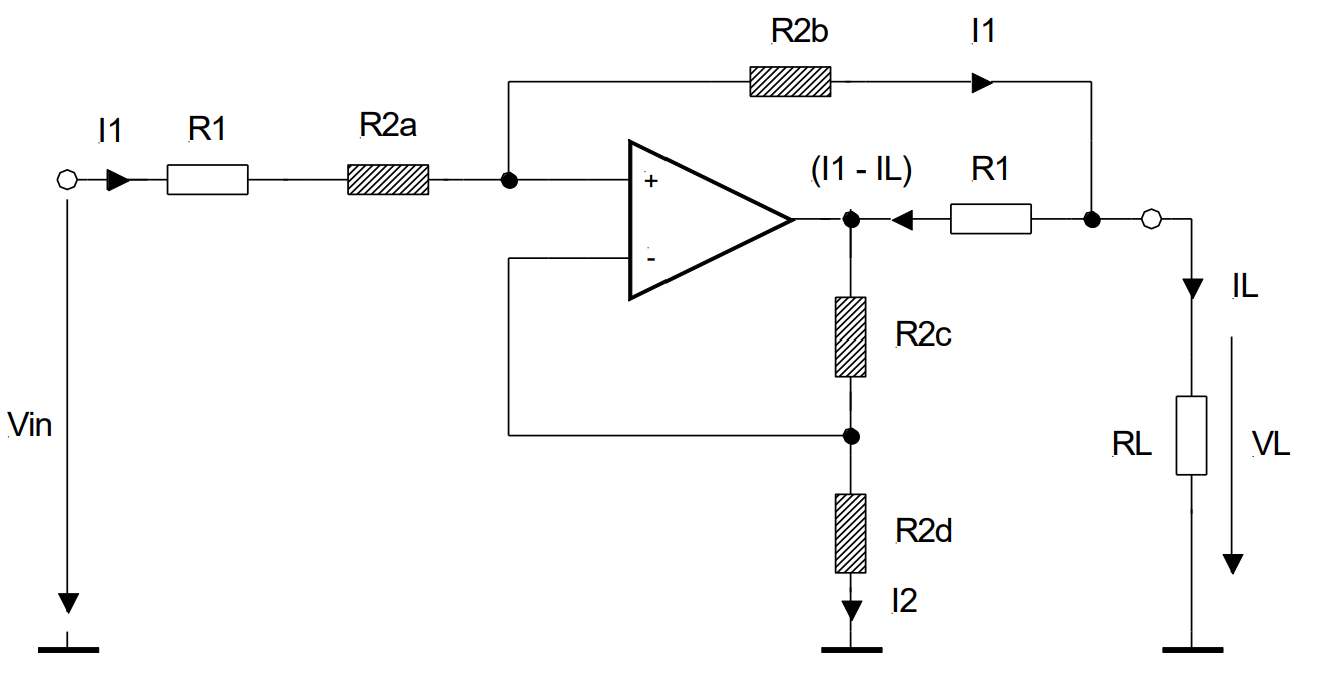
\includegraphics[width = 3.5cm]{img/OpAmp/Spannungsgesteuerte_Stromquelle_geerdete_Last.png} &
    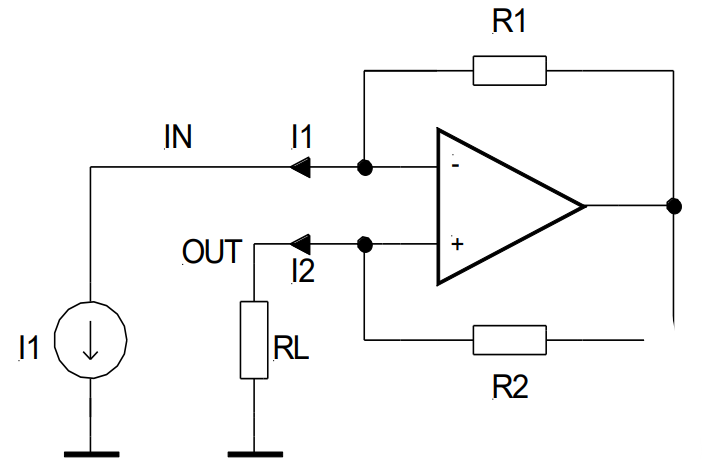
\includegraphics[width = 3.5cm]{img/OpAmp/Stromgesteuerte_Stromquelle.png}                     \\
    $ I_L = \frac{V_{in}}{R_1} $                                                                 &
    $ I_L = \frac{V_{in}}{R_S} $                                                                 &
    $ I_L = \frac{V_{in}}{R_1} $                                                                 &
    $ R_1I_1=R_2I_2; \; A_i = \frac{I_2}{I_1} = \frac{R_1}{R_2}  $
  \end{tabularx}
\endgroup

\subsubsection{Filterschaltungen}
\begingroup
  \small
  \begin{tabularx}{0.8\textwidth}{p{155pt}p{155pt}p{155pt}}  \textbf{RC-Integrator}                    &
    \textbf{Differenzierer}                                                              &
    \textbf{Tiefpass-Filter}                                                               \\
    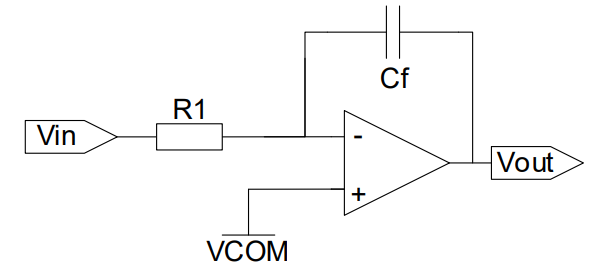
\includegraphics[width=3.5cm]{img/OpAmp/RC-Integrator.png}                           &
    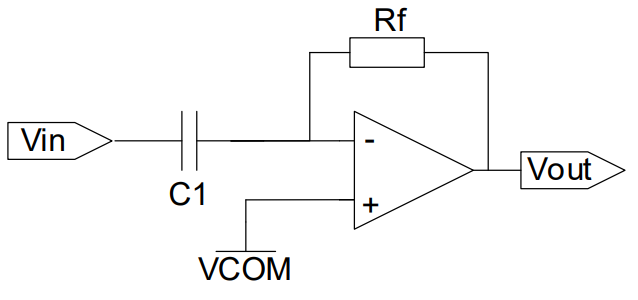
\includegraphics[width=3.5cm]{img/OpAmp/Differenzierer.png}                          &
    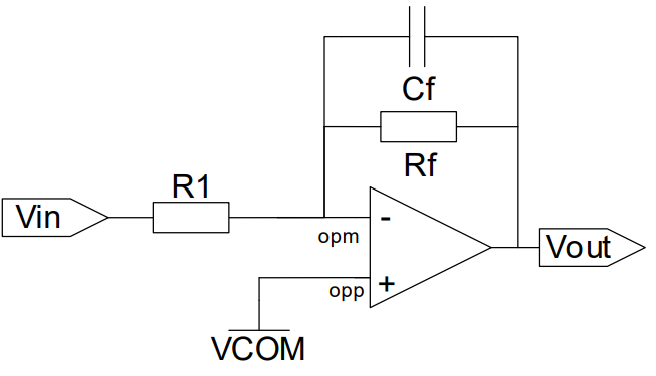
\includegraphics[width=3.5cm]{img/OpAmp/TiefpassFilter.png}                            \\
    $V_{out}(t) = -\frac{1}{C} \int \limits _0 ^t i_c(\tau) d\tau + V_c(t=0)$ \newline
    $V_{out}(t) = -\frac{1}{R \cdot C} \int \limits _0 ^t V_{in}(\tau) d\tau + V_c(t=0)$ &
    $ pen$                                                                               &
    \\
    \textbf{Bandpass-Filter}                                                             &
    \textbf{Allpass-Filter}                                                              &
    \\
    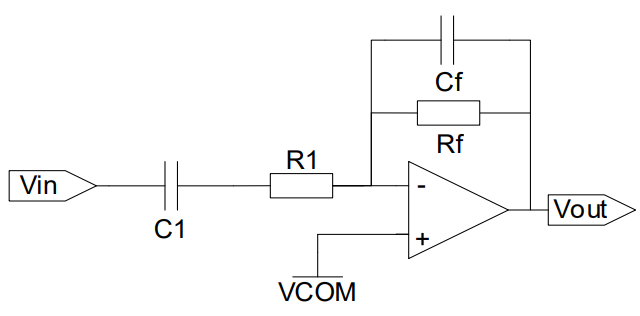
\includegraphics[width=3.5cm]{img/OpAmp/BandPass.png}                                &
    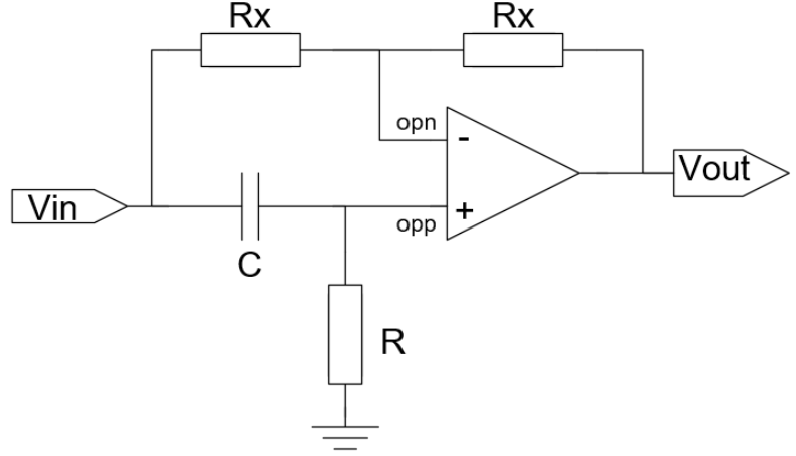
\includegraphics[width=3.5cm]{img/OpAmp/AllPass.png}                                 &
    \\
    $ asdf$
  \end{tabularx}
\endgroup
\subsection{Nicht ideale OpAmps}
Offset-Spannung
Eingans-ströme
Arbeitsbereiche
Begrenzte Verstärkung $A_ol$
\end{document}
